\chapter{Exploring the neuroprotective effects of tibolone during astrocytic metabolic inflammation: a flux balance analysis approach}
\begin{tabular}{rm{12cm}}
\textsf{\textbf{Written by:}} & \textit{Daniel Osorio, Janneth Gonzalez and Andrés Pinzón-Velasco}\\ 
\end{tabular}
\section*{Abstract:}
Inflammation is a complex biological response to injuries, metabolic disorders or infections and its dysregulation induces many complex diseases through astrocytic dysfunction. The increase of free saturated fatty acid produce a metabolic inflammation response, generally associated with the induction of diverse intracellular stresses, such as mitochondrial oxidative stress, endoplasmic reticulum stress, and autophagy defects.  Astrocytes respond to inflammation through a complex reaction called astrogliosis. During astrogliosis, glial cells generally associated with several beneficial activities in the CNS, also act as a source of inflammatory mediators and as generators of ROS that have the potential to damage neurons. In search of compounds with neuroprotective effects that imitate the neuroprotective actions of steroids without their prejudicial side effects; the synthetic neurosteroid Tibolone was identified. Although Tibolone has been shown to exert neuroprotective actions in cultured and under ischemia injury rat neurons, its specific actions on glial cells have received very little attention. Nevertheless, actually, is not well know the effects of tibolone on glial cells that allow its neuroprotective action. In this work, we model and simulate the metabolic inflammation response in mature astrocytes through Flux Balance Analysis (FBA), and explore the neuroprotective effects of tibolone under the inflamed state. We focused on identification of changes in metabolic pathways activation, functional products, gliotransmitter release and the neuroprotective effects mediated by tibolone over inflamed scenario. The generated network consisted of 1262 genes encoding for enzymes performing 2747 reactions distributed across eight compartments, which was studied using a constrained-based modeling approach to recreating three different scenarios in mature astrocytes (healthy, inflamed and medicated), and validated with available experimental evidence. From our analysis, we predict that tibolone execute their neuroprotective effects through a reduction of neurotoxicity mediated by L-glutamate in astrocytes.
\section{Introduction}
\subsection*{Astrocyte-Neuron Metabolic Relationships}
Astrocytes are the most abundant cells in the human brain and play important roles in the central nervous system (CNS) \cite{Takuma2004}. They are highly associated with several homeostatic functions such as glutamate, ion, and water homeostasis, energy storage in the form of glycogen, synapse formation, and remodeling, defense against oxidative stress, scar formation, tissue repair and modulation of synaptic activity via the release of gliotransmitters \cite{Lange2012}. Astrocytes metabolize glucose in the anaerobic way to produce lactate, which is released to neurons through monocarboxylate transporters \cite{Kimelberg2010}. Lactate is used in neurons as an energy substrate after its conversion to pyruvate and subsequently to ATP via oxidative phosphorylation \cite{Allen2009}.\\

Astrocytes play an important role in glutamate-mediated synaptic activity \cite{Halassa2010}; according to the astrocyte–neuron lactate shuttle model, astrocytes respond to glutamate-induced activation by increasing their rate of glucose uptake and the release of lactate into the extracellular space, increasing the lactate available to be used by neurons to supply their energetic needs \cite{Giaume2010}. Glutamate is uptake by astrocytes through the glutamate-aspartate transporter and glial glutamate transporter-1, inducing events that involve the activation of Na$^+$–K$^+$-ATPase and maintaining extracellular glutamate at homeostatic levels \cite{Nijboer2013}. Part of incorporated glutamate is converted to glutamine through glutamine synthetase, which is only associated with glial cells and released to neurons using electroneutral systems-N transporters coupled to Na$^+$ and H$^+$ \cite{Barres2008}. In neurons, glutaminase enzyme converts glutamine back into glutamate which can be used again for neurotransmission or metabolized into the neuronal Krebs cycle \cite{Shen2013}.\\

Astrocytes uptake and release many other substances related to synaptic transmission \cite{Petrelli2016}. However D-serine, a neurotransmitter that acts as a co-agonist with glutamate at NMDA receptors is one of the most important \cite{Halassa2010}. Due in the brain, only glial cells can synthesize serine, all available D-serine at synapsis is associated to be primarily produced and secreted by astrocytes \cite{Barres2008}. D-serine is synthesized in astrocytes by serine racemase from L-serine \cite{Durrant2014}. Serine and glycine are involved in a cycle between astrocytes and neurons similar to the glutamate-glutamine cycle \cite{Cakir2007}. Additionally, to these energetic and synaptic support associated functions, astrocytes also play an important role in the reduced glutathione (GSH) metabolism of the brain \cite{Raps1989}. GSH is the major cellular antioxidant and plays an important neuroprotective role \cite{Jha2016}. Cellular GSH levels are closely correlated with cell survival under adverse conditions \cite{Allaman2011}; it is synthesized from glutamate, cysteine, and glycine and releases directly from astrocytes through GSH transporters ion-independent in a concentration gradient dependent transport \cite{Wang2000}. \\

This strong metabolic cooperation between astrocytes and neurons allows predicting that even a small astrocytic dysfunction might cause and/or contribute neurodegenerative processes \cite{Maragakis2006}. Homeostatic astrocyte function is required for neuronal survival after different brain insults, such as inflammation, glucose deprivation, traumatic brain injury and ischemia \cite{Avila-Rodriguez2014,Jha2016}. Astrocytes protect neurons of the most important factors that contribute to neuronal cell death such as glutamate-mediated excitotoxicity leading to disturbances in calcium and sodium intracellular metabolism, mitochondrial dysfunction, oxidative stress, cytokines and toxins \cite{Takuma2004,Lange2012,Nijboer2013,Hussain2013}.

\subsection*{Astrocytes response to Inflammation}
Inflammation is a complex biological response to injuries, metabolic disorders or infections, and its dysregulation induces many complex diseases through astrocytic dysfunction \cite{Masel2010,Yan2013,Jha2016}. In the brain, inflammatory response acts as a defense mechanism against any threat to homeostatic state inducing changes in glucose metabolism and release of pro-inflammatory factors \cite{Allaman2011}. Inflammation responses in CNS are mediated by glial cells that acquire reactive phenotypes to participate in repair mechanisms \cite{Takuma2004,Fitch2008,Jha2016}. \\

Astrocytes, as glial cells are highly sensitive cells to inflammatory mediators, they respond to inflammation through a complex reaction named astrogliosis \cite{Dowell2009a}. During astrogliosis, glial cells generally associated with several beneficial activities in the CNS, also act as a source of inflammatory mediators and as generators of reactive oxidant species (ROS) that have the potential to damage neurons \cite{Molofsk2012}. Astrogliosis is characterized by a low regulation of mitochondrial dynamics that result in mitochondrial failure \cite{Sidoryk-Wegrzynowicz2013}. Mitochondrial failure induces the deregulation of Ca$^{2+}$ homeostasis and increased ROS generation, both of which are linked to neurotoxicity \cite{Lange2012}. At metabolic level, inflammatory process has been associated with an increase of free saturated fatty acid in comparison with healthy conditions in some brain tissues \cite{Gupta2012}. \\

The increase of free saturated fatty acid induce metabolic inflammation, a response associated with the induction of diverse intracellular stresses, such as mitochondrial oxidative stress, endoplasmic reticulum stress, and autophagy defects \cite{Jha2016}. Lipid excess in metabolic inflammation activates IKK$\beta$ and NF-$\kappa\beta$ signaling pathways, which ultimately impairs leptin and insulin hormonal signaling and further triggers the synthesis and release of increased amounts of ROS and pro-inflammatory cytokines (TNF-$\alpha$ and IL-6) from glial cells to sustain the neuroinflammatory state \cite{Purkayastha2015}. Enhanced ROS generation by reactive glial cells trigger mitochondria dysfunction in neuron, which induces neuronal apoptosis, the prerequisite for a diverse number of neurodegenerative conditions \cite{K.2006}.

\subsection*{In silico Systems Biology and  Inflammation}
Inflammatory pathways are evolutionarily conserved, complex, redundant and interconnected \cite{Vodovotz2010} . These characteristics difficult each attempt to understand any disease having inflammation as its core using the traditional reductionism-based scientific method and the current regulatory framework \cite{Vodovotz2008}. Traditional methods generally focus on single molecules and genes as the targets of study and potential therapy development, nevertheless, mechanistic simulation through a translational systems biology methods allows lead to an understanding of the origin of patterns based on `omic' data integration in order to facilitate the design of novel therapies  \cite{An2011}.\\

Inflammation is a complex system, which is characterized by sensitivity to initial conditions, positive and negative feedback loops, combined robustness and fragility, and the emergence of nonintuitive behaviors \cite{Mi2010}. Translational Systems Biology to inflammation is focused on simulated clinical trials, trying to progress toward personalized diagnostics, personalized medicine, and the rational design of drugs \cite{Vodovotz2010}.

\subsection*{Tibolone}
Drugs as steroids compounds are the most potent and effective agents in controlling chronic inflammatory diseases \cite{Laveti2013}. However, steroids prescription is limited due to their adverse side effects \cite{Albertazzi1998}. Some steroids synthesized in the nervous system, called ‘neurosteroids’, display beneficial neuroprotective properties, which may be of particular importance in the treatment of diseases where inflammation and neurodegeneration is predominant including age-dependent dementia, stroke, epilepsy, spinal cord injury, Alzheimer’s disease (AD) and Parkinson’s disease (PD) \cite{Wojtal2006}. \\

Neuroprotective actions of molecules that may imitate the neuroprotective actions of steroids without the prejudicial side effects, such as selective estrogen receptor modulators (SERMs) and selective tissue estrogenic activity regulators (STEARs) have been tested in previous studies \cite{Kloosterboer2001,Sharma2006}. Tibolone is a compound, traditionally used as hormone replacement therapy in post-menopausal women \cite{Timmer2002}, that has been shown neuroprotective effects in cultured and under ischemia injury rat neurons \cite{Altinoz2009}.\\

Tibolone is a synthetic steroid drug with estrogenic, progestogenic, and weak androgenic actions; is metabolized in three compounds, two major active metabolites, 3$\alpha$-hydroxy tibolone and 3$\beta$-hydroxy tibolone acting as potent agonists of the estrogen receptor (ER) and its metabolite $\Delta$4tibolone acting as agonists of the progesterone and androgen receptors \cite{Kloosterboer2004}. Tibolone and their metabolites have tissue selective action mechanisms (progestogenic, androgenic and estrogenic) reported in liver, bone, breast and brain according to receptor interaction and activation \cite{Kloosterboer2001}. Nevertheless, actually, is not well know the effects of tibolone on glial cells that allow its neuroprotective effects \cite{Avila-Rodriguez2014}. Previous studies have shown that 3-hydroxy-metabolites of tibolone exert agonistic actions on human astrocytes through the activation of estrogen receptors, indicating that astrocytes are a target for tibolone \cite{Altinoz2009}.\\

In this work, we simulate the metabolic inflammatory response in mature astrocytes caused by the increased uptake of palmitate, the most common free saturated fatty acid. We model and simulate the metabolic response using a translational system biology approach called Flux Balance Analysis (FBA) described in methods. We focused on the identification of changes in metabolic pathways activation, functional products, gliotransmitter release and the neuroprotective effects mediated by tibolone in the inflamed scenario.
\section{Material and Methods}
\subsection*{Tissue Specific Model Construction}
The tissue specific model construction process started with the identification of all enzyme‐coding genes expressed over the mean in at least 50\% of samples for healthy human astrocytes indexed in the GEO database \cite{Edgar2002} as GSE73721 \citep{Zhang2016}. Gene identifier conversion from GeneCards\cite{rebhan1997genecards} to ENTREZ \cite{maglott2005entrez} was performed through `UniProt.ws' R Package \cite{Carlson2016}. Reactions associated with the identified genes were mapped from the Human Genome-Scale  Metabolic Reconstruction RECON 2.04 downloaded from the VMH Lab (https://vmh.uni.lu) \cite{thiele2013community}. The R package `g2f' \cite{G2F} was used to identify and fill the gaps using all no gene-associated reactions included in RECON 2.04, as well as to identify and remove all blocked reactions  from the reconstruction.\\

All reactions involved in the conversion of extracellular glutamate, glycine, cysteine and glucose to extracellular glutamine, glycine, serine-D, reduced glutathione, lactate, and ATP respectively were added. Exchange reactions were limited to components of the Dulbecco's Modified Eagle Medium (DMEM) as input and gliotransmitters (glutamine, D-serine, ATP, glutamate), reduced glutathione, lactate, glucose, nitric oxide, prostaglandins and leukotrienes as output. Finally, syntax, mass-charge validation and creation of SBML files were carried out through the `minval' R Package \cite{MINVAL}. Reaction limits (upper and lower bounds) were constrained proportionally to the mean gene expression reported for genes included in Gene-Protein-Reaction (GPR) \cite{Thiele2010} associated to each reaction in samples of 47 to 63 years old using the `exp2flux' R package \cite{EXP2FLUX}. All Flux Balance Analysis (FBA) were performed using the `sybil' \cite{Gelius-Dietrich2013} R Package running under R 3.3.1 \cite{RCoreTeam2016}.
\subsection*{Flux Balance Analysis}
FBA is a linear optimization method for simulating metabolism that allows identifying the set of reactions involved in the production of a biological response within a metabolic model \cite{Orth2010}. The metabolic reactions are represented internally as a stoichiometric matrix ($S$), of size $m \times n$, where $m$ represents the compounds and $n$ the reactions; the entries in the matrix are the stoichiometric coefficients of the metabolites participating in a reaction \cite{Raman2009}. The flux through all of the reactions in a network is represented by the vector $v$, which has a length of $n$. The concentrations of all metabolites are represented by the vector $x$, with length $m$. The systems of mass balance equations at steady state, $\dfrac{d_{x}}{d_{t}}=0$ or $S \times v = 0$. FBA seeks to maximize or minimize an objective function which can be any linear combination fluxes, to obtain a flux for each reaction, indicating how much each reaction contributes to the objective function \cite{Orth2010}.

\begin{table}[h]
\caption{Main metabolic capabilities associated to astrocytes represented as the set of objective functions used to evaluate neuroprotective effects of Tibolone under inflamed scenarios}
\label{OF}
\begin{center}
\begin{tabular}{rm{6.5cm}m{6cm}}
\hline
ID & FORMULA REACTION & DESCRIPTION \\
\hline
\hline
Glu2Gln & 1 glu\_L[e] $\Rightarrow$ 1 gln\_L[e] & Glutamate - Glutamine Cycle \\
Gly2SerD & 1 gly[e] $\Rightarrow$ 1 ser\_D[e] & Glycine to D-serine conversion\\
Glc2Lac & 1 glc\_D[e] $\Rightarrow$ 2 lac\_L[e]& Lactate production from Glucose \\
Glc2ATP & 1 glc\_D[e] $\Rightarrow$ 36 atp[e] & ATP production from Glucose \\
Cys2GTHRD&1 cys\_L[e] + 1 glu\_L[c] + 1 gly[c] $\Rightarrow$ 1 gthrd[e]& Catch of Cysteine to produce reduced Glutathione \\
\hline
\end{tabular}
\end{center}
\end{table} 

FBA for healthy, inflammated and medicated scenarios was resolved using GLPK 4.60, setting the generic human biomass reaction included in RECON 2.04 and each one of reactions described in table \ref{OF} as objective functions. Models were analyzed by comparing fluxes between scenarios, metabolites production rate and a sensitivity analysis.
\subsection*{Metabolic Scenarios}
To test neuroprotective effects of tibolone during astrocytic metabolic inflammation we define three different metabolic scenarios. A `healthy' scenario, where palmitate uptake rate was freely set by optimizer; an `inflamed' scenario, where uptake rate of palmitate was forced to be stable in the mean of the half maximal inhibitory concentration (IC50) value for all objective functions included in table \ref{OF}. IC50 values were calculated through a robustness analysis performed using uptake of palmitate (`EX\_hdca(e)' in RECON 2.04) as control reaction and 1000 points in the range from 0 to 1 mMgDW$^{-1}$h$^{-1}$ for each objective function. Uptake value where each objective function reached IC50 was selected and subsequently averaged. Finally, a medicated scenario, defined as an inflamed scenario that includes 279 reactions associated with estradiol-derivated compounds and ten specific reactions associated with Tibolone action mechanism not included in RECON 2.04 described in table \ref{Tibolone}.

\begin{table}[h]
\caption{Set of reactions added to recreate the medicated scenario model over the astrocyte tissue-specific model. Reactions are the representation of tibolone metabolism in the brain following the reported by Kloosterboer (2004).}
\label{Tibolone}
\begin{center}
%\footnotesize{
\begin{tabular}{rlm{7cm}}
\hline
ID & FORMULA REACTION & DESCRIPTION \\
\hline
\hline
T1 & tibolone[e] $\Leftrightarrow$ & Tibolone exchange reaction\\
T2 & tibolone[e] $\Leftrightarrow$ a3OHtibolone[e] & 3$\alpha$hidroxytibolone interconvertion\\
T3 & tibolone[e] $\Leftrightarrow$ b3OHtibolone[e] & 3$\beta$hidroxytibolone interconvertion \\
T4 & tibolone[e] $\Rightarrow$ d4tibolone[e] & $\Delta$4tibolone isomer formation \\
T5 & b3OHtibolone[e] $\Rightarrow$ d4tibolone[e] &  $\Delta$4tibolone isomer formation from 3$\beta$-hidroxytibolone \\
T6 & a3OHtibolone[e] $\Rightarrow$ estradiol[c] & Estradiol receptor agonist action mechanism of 3$\alpha$-hidroxytibolone\\
T7 & b3OHtibolone[e] $\Rightarrow$ estradiol[c] & Estradiol receptor agonist action mechanism of 3$\beta$-hidroxytibolone\\
T8 & d4tibolone[e] $\Rightarrow$ prgstrn[c] + tststerone[c] & Progesterone and androgen receptor activation by tibolone $\Delta^4$ isomer\\
T9 & a3OHtibolone[e] $\Leftrightarrow$ a3SOtibolone[e] & 3$\alpha$hidroxytibolone interconvertion to sulfated inactive compounds \\
T10 & a3SOtibolone[e] $\Rightarrow$ & Tibolone inactive form in blood \\ 
\hline
\end{tabular}
\end{center}
\end{table} 

\subsection*{Metabolic Changes}
Metabolic changes across metabolic scenarios were measured through two different approximations. Flux differences for each reaction between optimized scenarios were measured using the fold change calculated as described in equation \ref{fC}.
\begin{ceqn}
\begin{align}
\label{fC}
   foldChange = \dfrac{valueModel2-valueModel1}{\left|valueModel1\right|}
\end{align}
\end{ceqn}

\subsection*{Pro-inflammatory, Anti-inflammatory and Tibolone Action Mechanism Associated Enzymes}
Enzymes involved in pro-inflammatory and anti-inflammatory responses as well as in the tibolone action mechanism were identified through sensitivity analysis as follows: Pro-inflammatory enzymes, are those that catalyze reactions that being knocked out allows an increase of objective function value. Anti-inflammatory enzymes are those associated with reactions that have a fold-change greatest equal to 2, and at being knocked out reduce even more the objective function value. Tibolone action mechanism associated enzymes are those that catalyze reactions that being knocked out inhibit entirely the metabolic effect of tibolone.

\section{Results}
All data, code, software and output files used in the developing of this work, are available to be downloaded from GitHub URL: https://github.com/dosorio/masterThesis as a free repository.

\subsection*{Tissue Specific Metabolic Model}
Generated astrocyte tissue-specific model describe the metabolism of 1956 compounds in a total of 2747 biochemical reactions associated to 1262 unique genes. Biochemical reactions include 60 exchange and 1080 transport reactions (79\% gene associated, facilitated or active transport) as is shown in figure \ref{Reactions}\textbf{A}.  
\begin{figure}[h]
\begin{center}
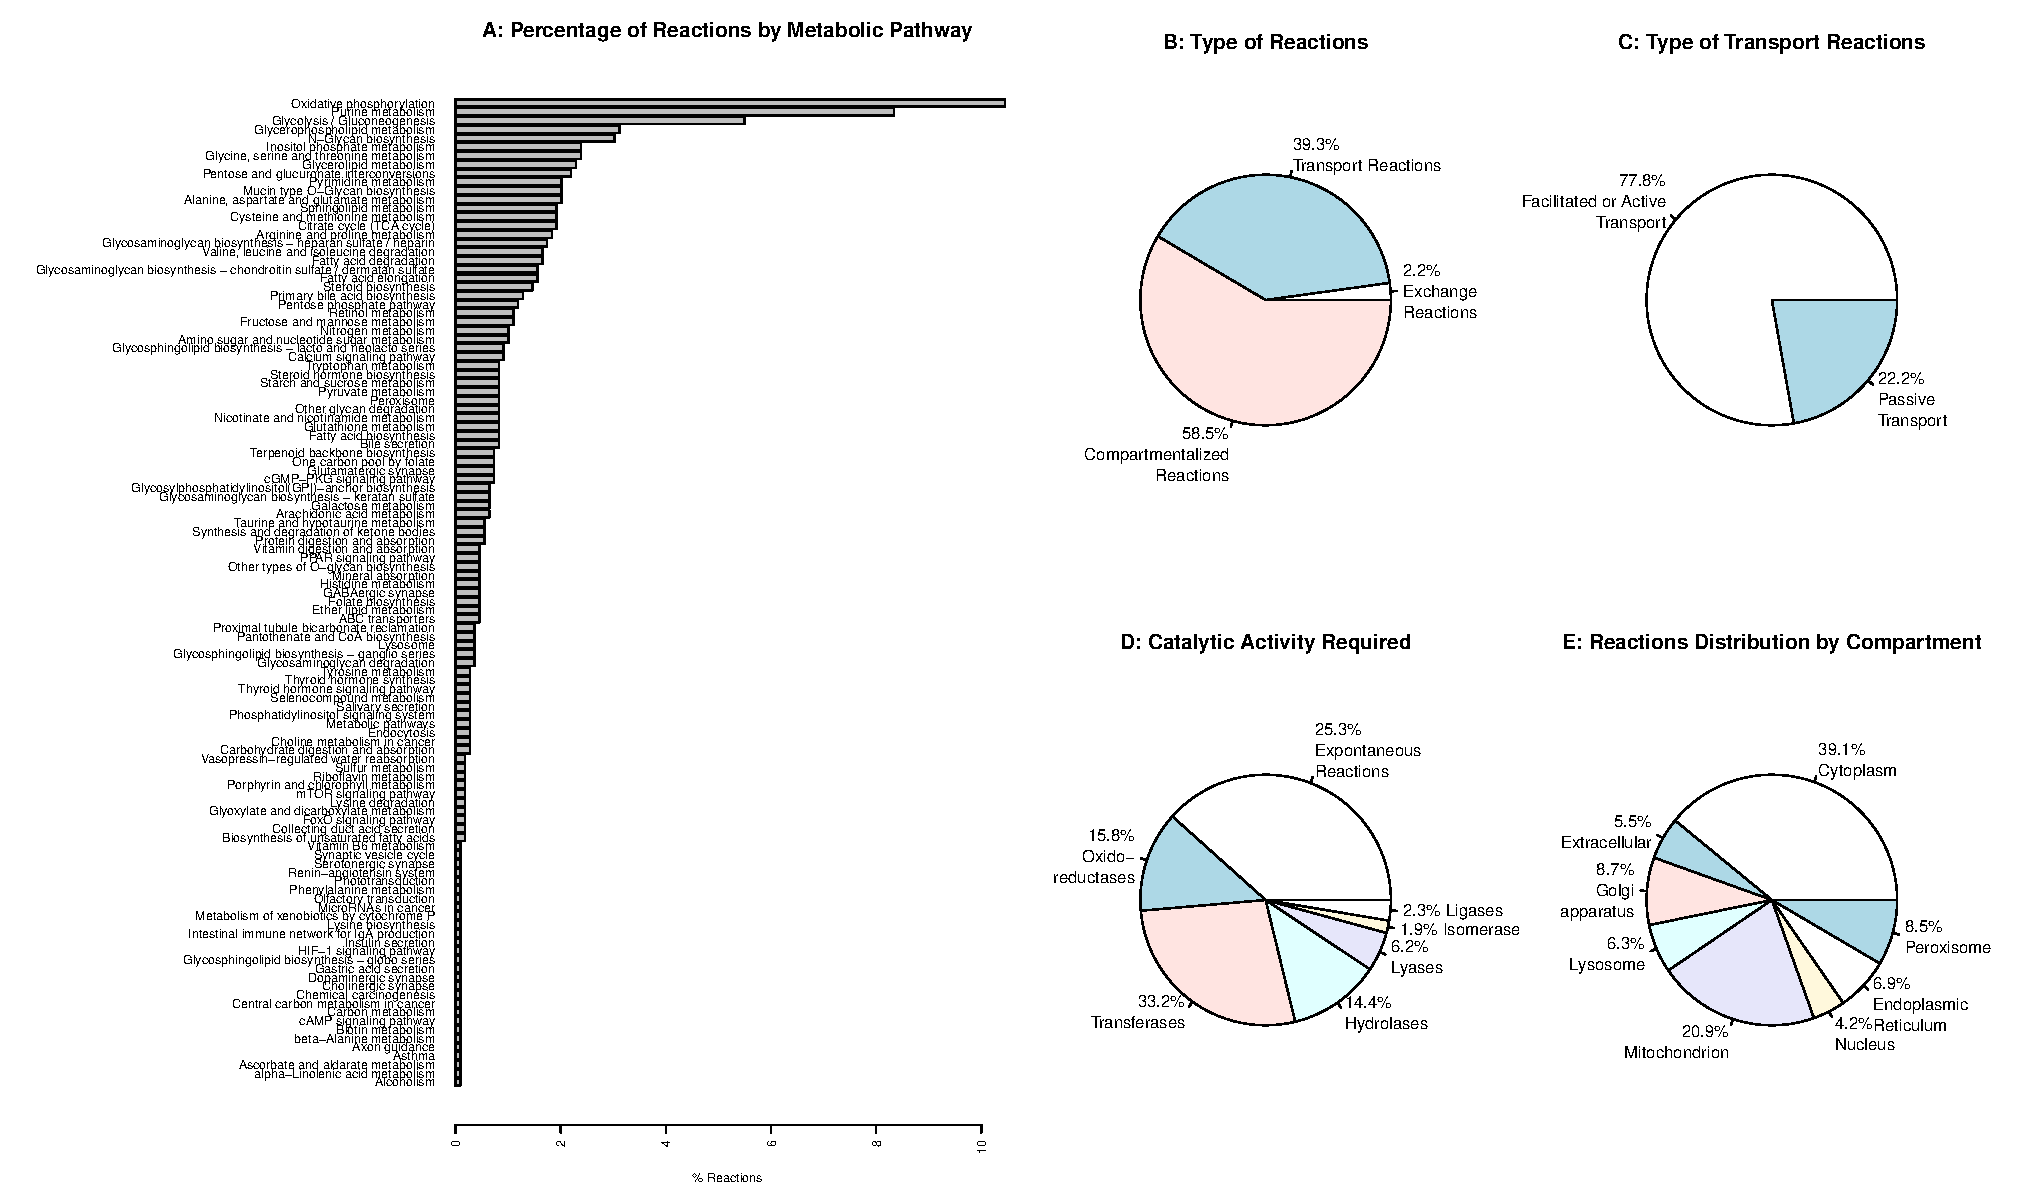
\includegraphics[width=\textwidth]{neuroprotective/RXN}
\end{center}
\caption{Distribution of biochemical reactions included in the astrocyte tissue-specific metabolic model, classification based in \textbf{A:} Type of reaction, \textbf{B:} Catalytic activity required and \textbf{C:} Associated compartment.}
\label{Reactions}
\end{figure}
To describe the astrocyte tissue-specific metabolic model, reactions were classified on the basis of required enzymatic activity to be catalyzed according to their Enzyme Commission (E.C) numbers (Fig. \ref{Reactions}\textbf{B}), sub-cellular locations according to metabolites compartment (Fig. \ref{Reactions}\textbf{C}), and metabolic pathways assigned in the KEGG database (Fig. \ref{Pathways}).  Based on the associated enzyme to each biochemical reaction 33.2\% of them are catalyzed by a transferase enzyme, 15.8\% by an oxidoreductase, 14.4\% by a hydrolase, 6.2\% by a lyase, 2.3\% by a ligase, 1.9\% by an isomerase enzyme and 25.3\% of them are spontaneous reactions without enzyme or gene associated. 
\begin{figure}[h]
\begin{center}
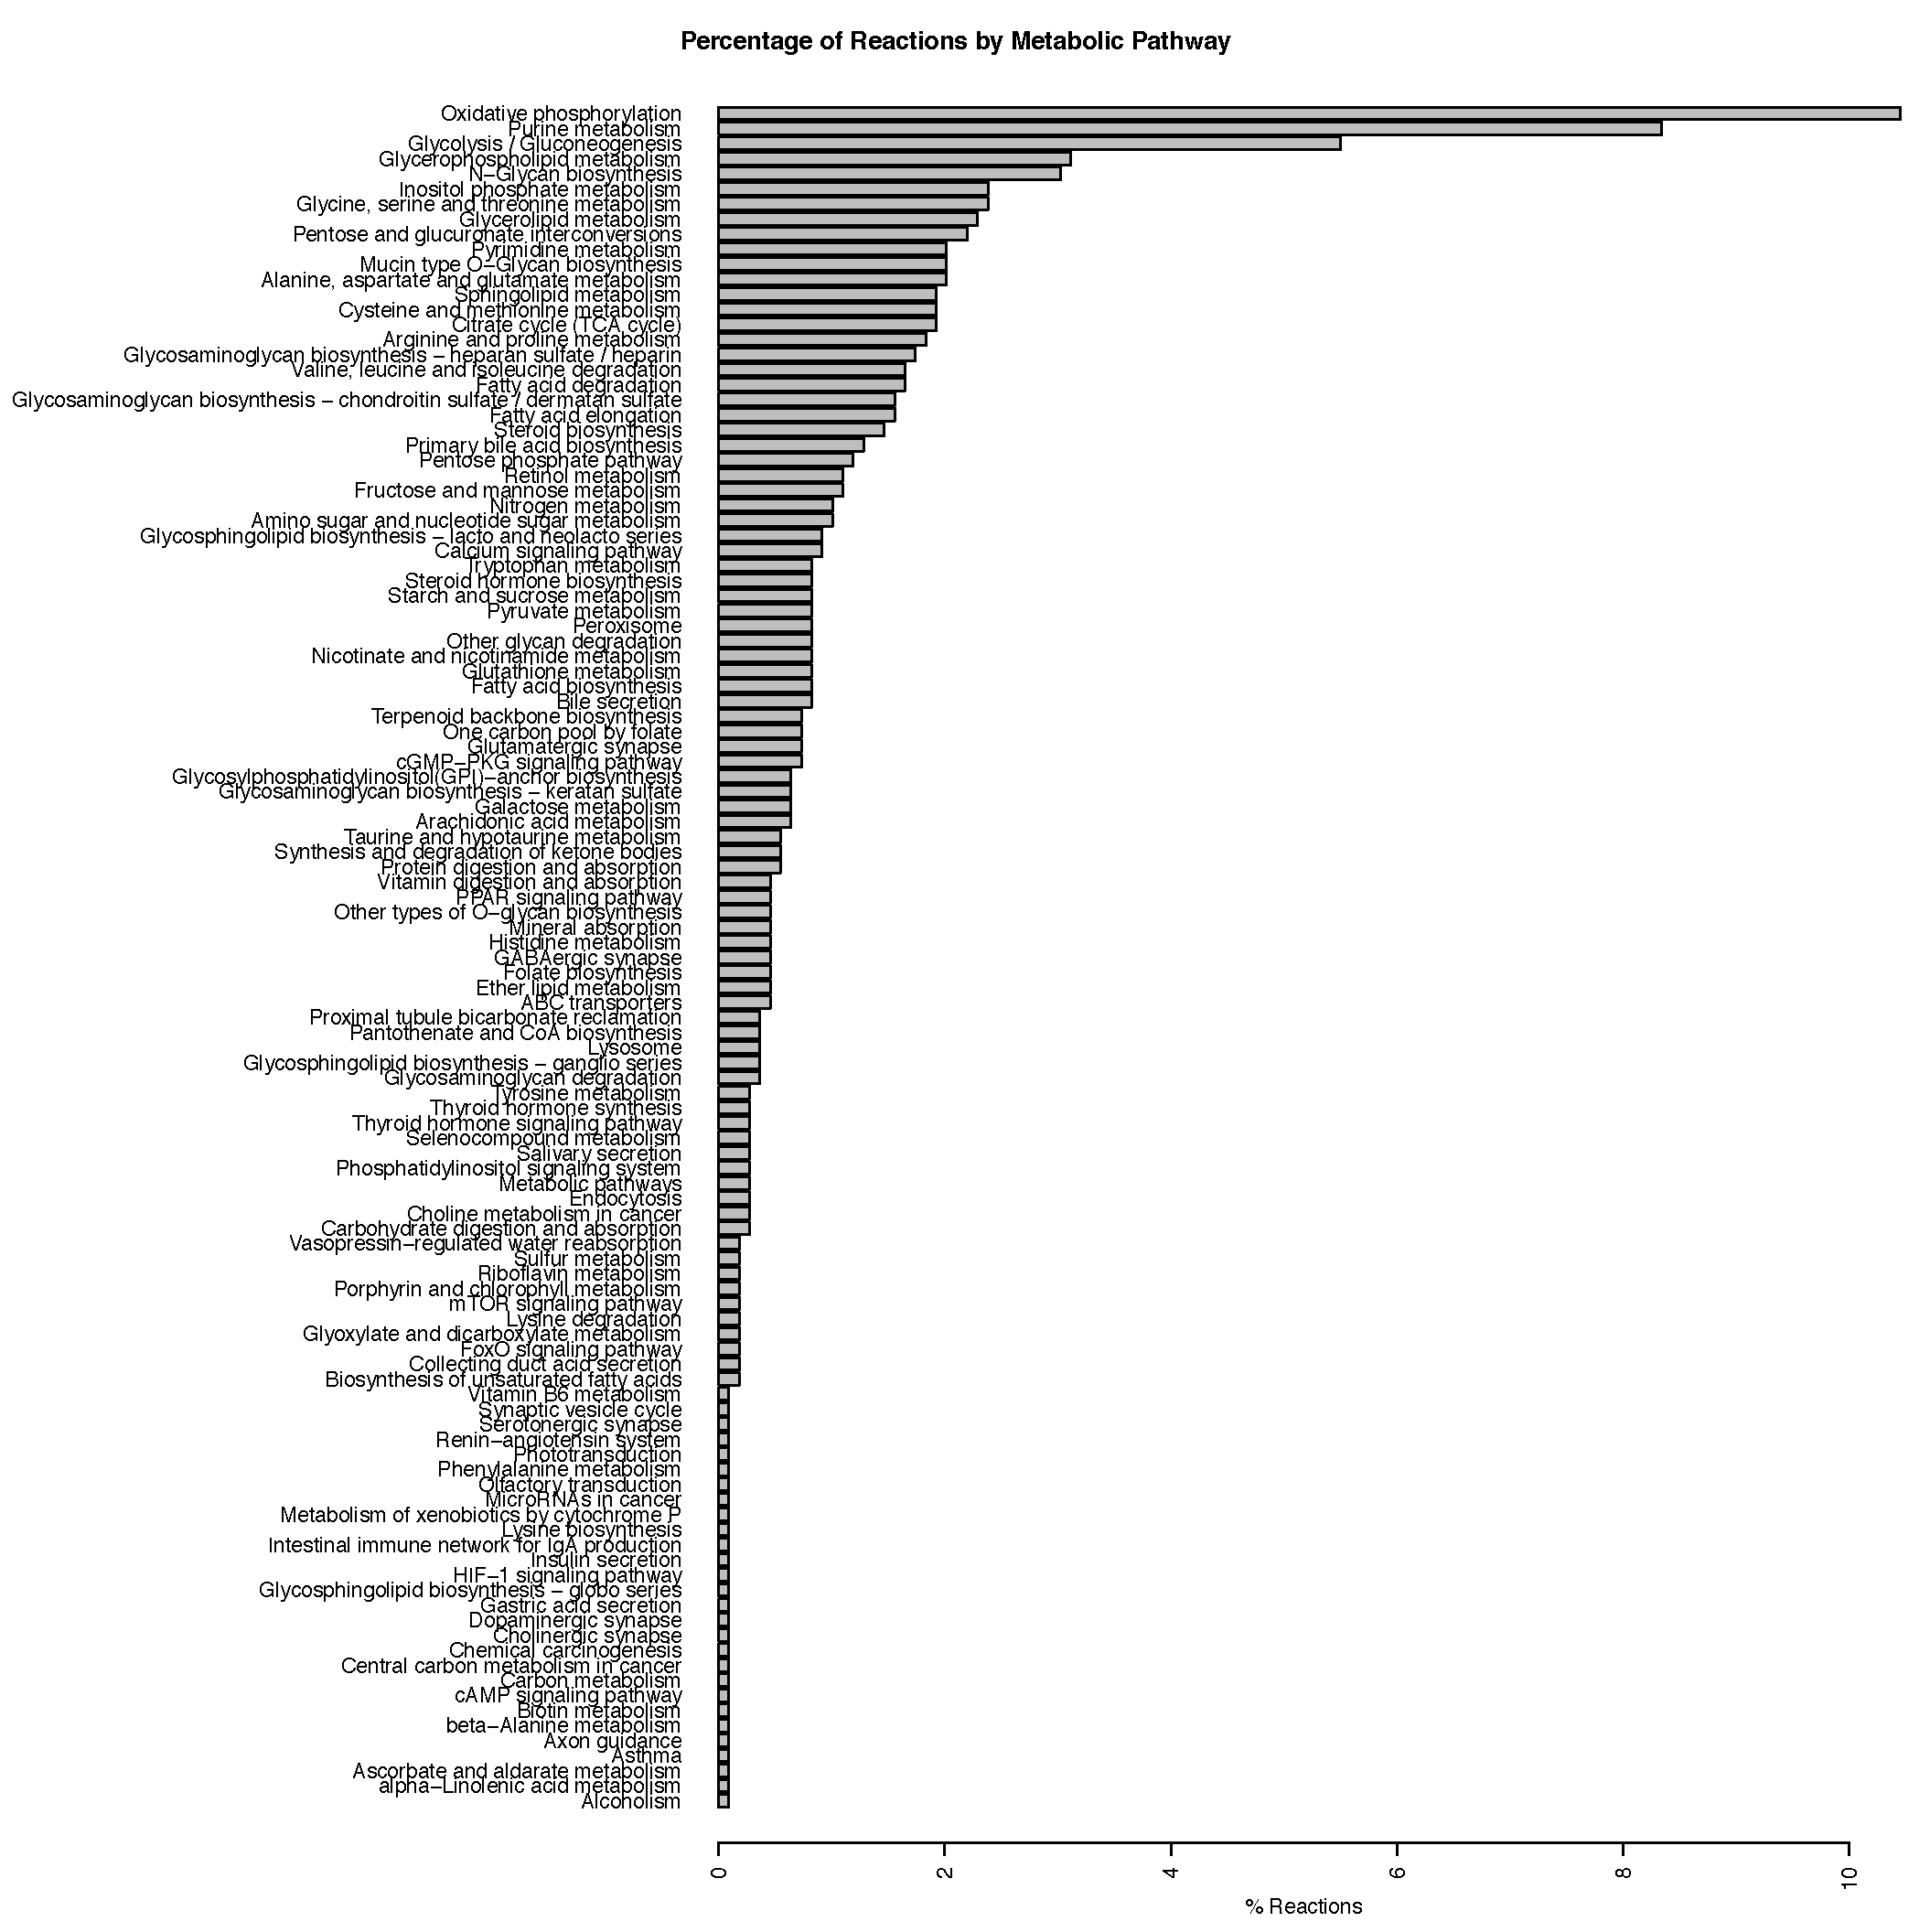
\includegraphics[width=0.6\textwidth]{neuroprotective/Pathways}
\end{center}
\caption{Pathways associated with biochemical reactions included in the astrocyte tissue-specific metabolic model. Pathway association was assigned based in the categorization of the KEGG database.}
\label{Pathways}
\end{figure}
In the classification shown in figure \ref{Reactions}\textbf{C}, the cytosolic and mitochondrial reactions contributed to 60\% of the total reactions in the model. The other 40\% of reactions are distributed in six other compartments as follows: 8.7\% occurs in Golgi apparatus, 8.5\% in the peroxisome, 6.9\% in the endoplasmic reticulum, 6.3\% in the lysosome, 4.2\% in nucleus, finally 5.5\% of them occurs outside the cell, in the extracellular space.
Reactions included in astrocyte model are associated with 113 metabolic pathways reported in the KEGG database \cite{Kanehisa2000}. Almost 50\% reactions are associated to 10 main metabolic pathways, highly related to astrocytes metabolism and neuron support metabolic functions \cite{Fitch1997,Ciccarelli2001,Cakir2007,Giaume2010, Sertbas2014, Sa2016}. Entirely distribution of reactions in metabolic pathways is shown in figure \ref{Pathways}. 
\subsection*{Healthy Scenario}
As previously reported by the Das \emph{et al.} wet lab, healthy human astrocytes grow up in DMEM culture medium \cite{Das2010}. Our metabolic simulation allows to predict an astrocytes slow grow rate  (0.37 mMgWD$^{-1}$h$^{-1}$) under DMEM medium.

\begin{figure}[h]
\begin{center}
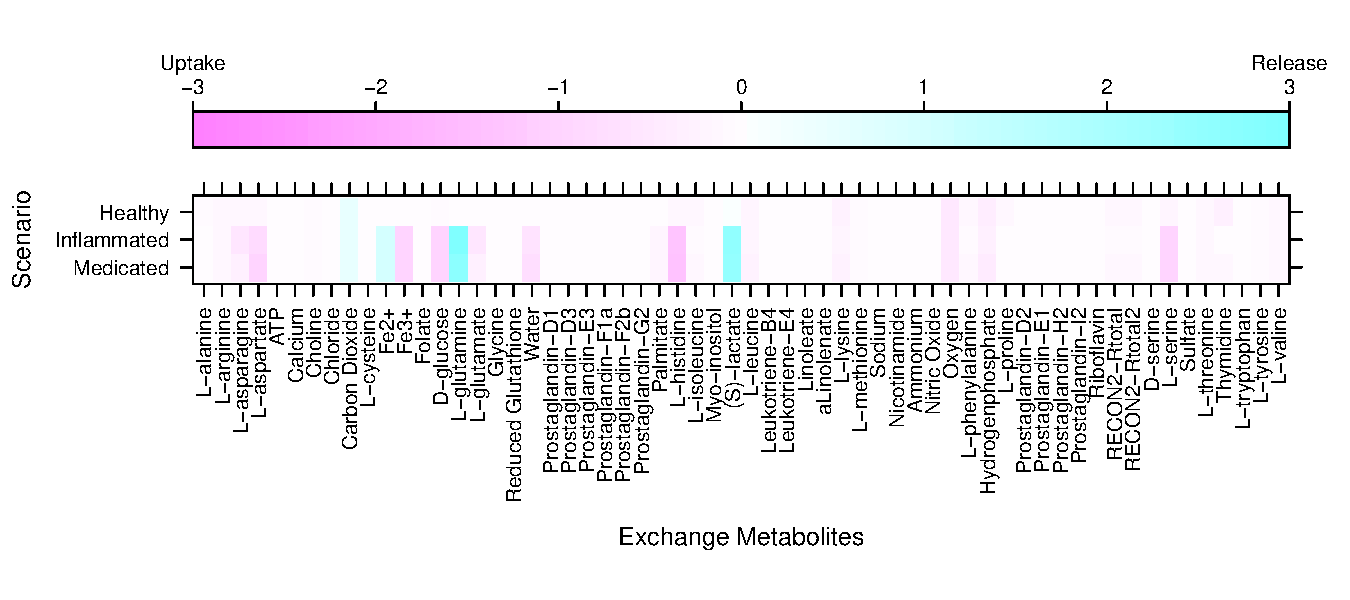
\includegraphics[width=\textwidth]{neuroprotective/Exchanges}
\end{center}
\caption{The exchange rate of metabolites between metabolic scenarios using the generic biomass reaction included in RECON 2.04 as the objective function}
\label{Exchanges}
\end{figure}

In our healthy scenario (Fig. \ref{Exchanges}), astrocytes activate the 52\% of model reactions and prefer a glucose-based metabolism, equal than found by Çakir \emph{et al.} and Bhowmick \emph{et al.} in resting conditions \cite{Cakir2007,Bhowmick2015}. Glucose is catabolized and constitutively released by astrocytes as lactate without any stimuli \cite{LeFoll2016}. This observation is highly expected due astrocytes release large amounts of lactate in the extracellular space which can be used by neurons to supply their energy needs \cite{Allaman2011}.  In our simulations, other gliotransmitters are synthetized and released by astrocytes only under specific stimulus (objective functions) and their release rate was used as a reference to the comparison between scenarios (Fig. \ref{Effects}).

\subsection*{Inflammated Scenario}
\begin{figure}[h]
\begin{center}
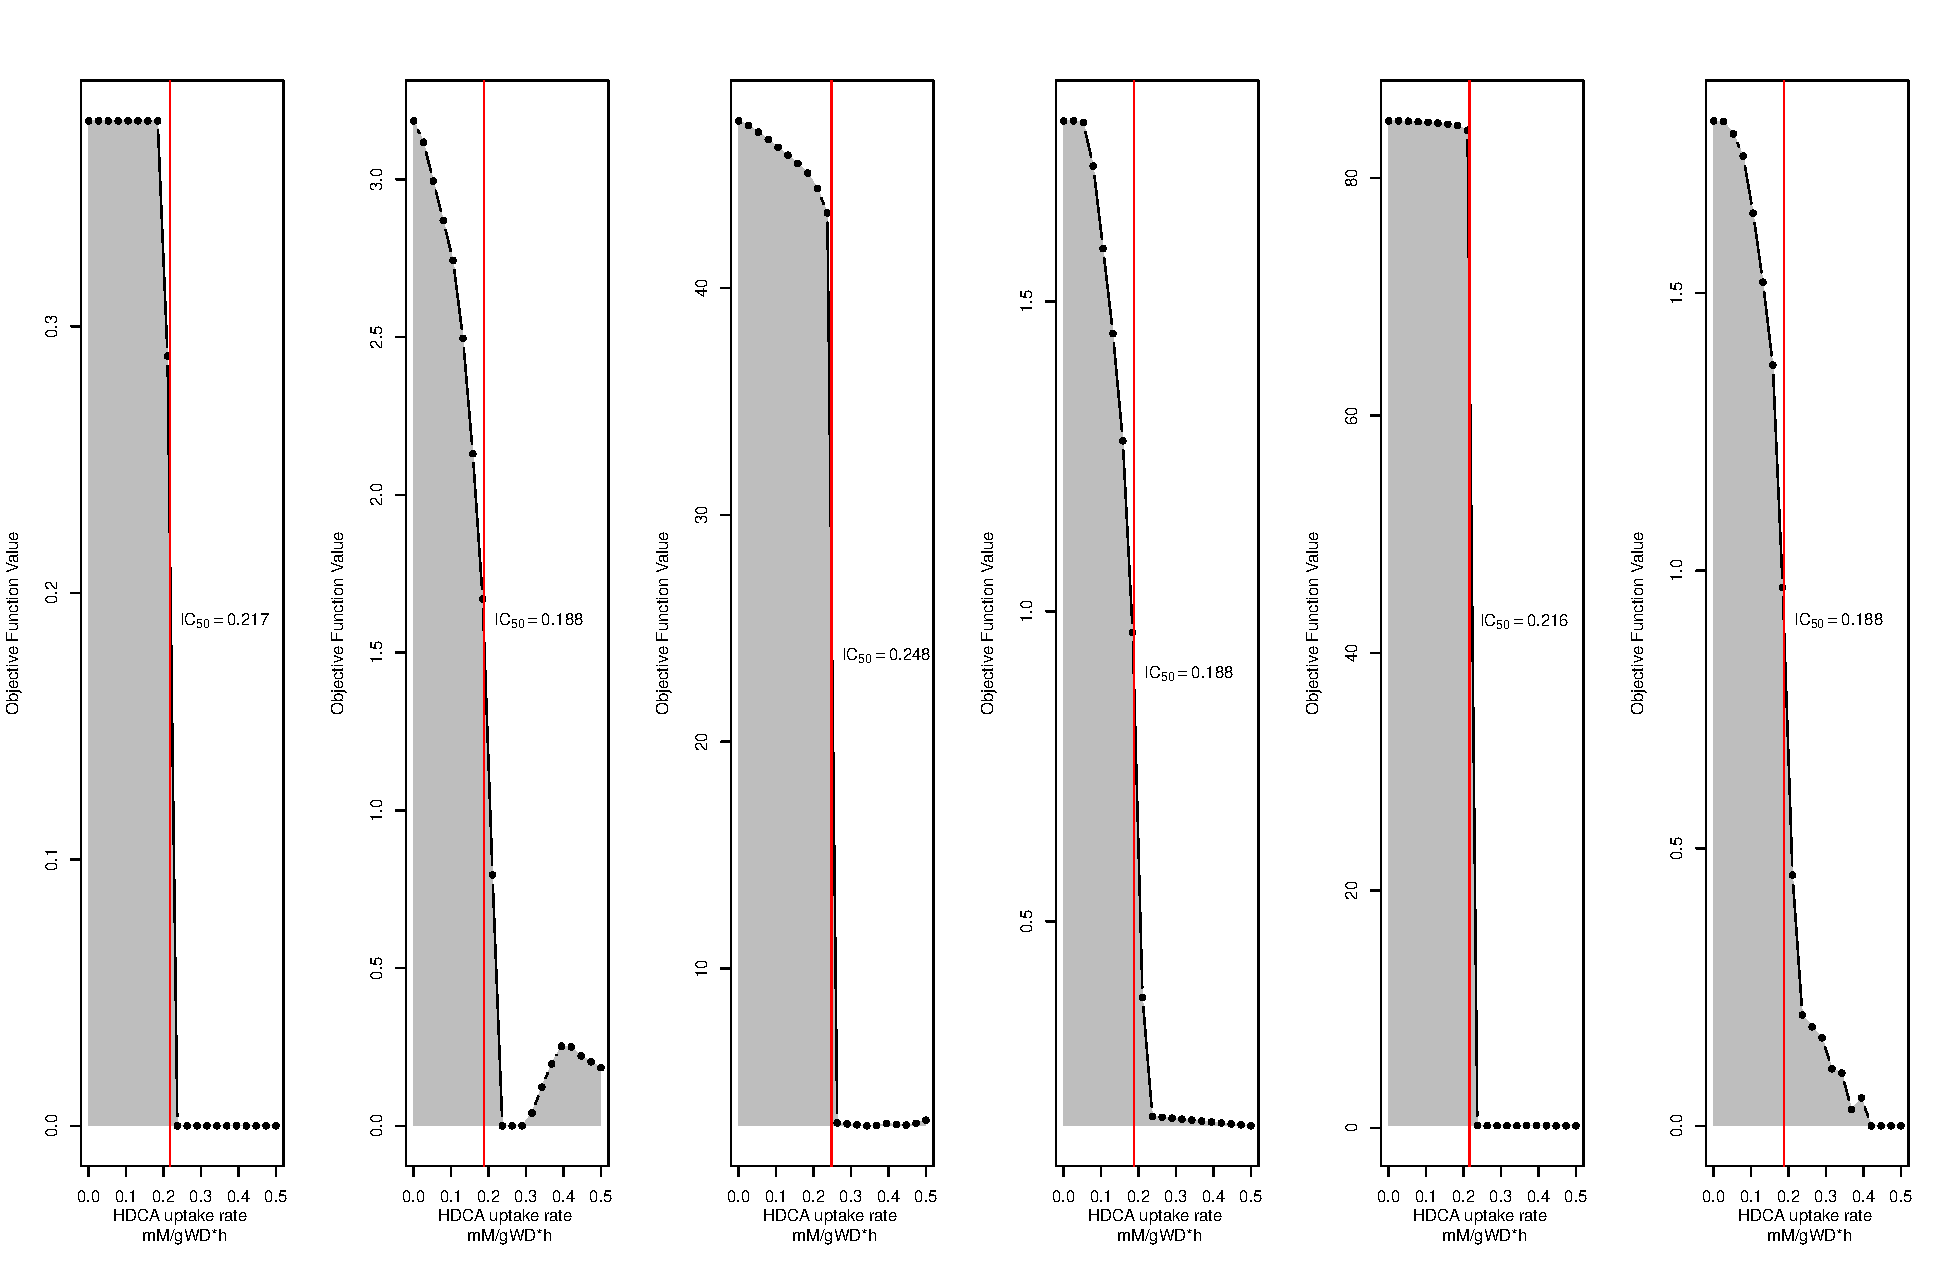
\includegraphics[width=\textwidth]{neuroprotective/IC50}
\end{center}
\caption{Robustness analysis to calculate palmitate-induced IC50 value for each objective function described in table \ref{OF}. The red line represents the calculated IC50 value.}
\end{figure}

In the model, the healthy scenario was perturbed to generate the inflamed scenario. The palmitate-induced IC50 value calculated for a set of metabolic functions (Table \ref{OF}) was 0.208 $\pm$ 0.024 mMgDW$^{-1}$h$^{-1}$. Calculated IC50 value is the same (0.2 mM) used by Liu \emph{et al.} in wet lab to induce an astrogliosis reaction \cite{Liu2013}. Inflammed scenario increases the demand for L-asparagine, L-aspartate, iron, D-glucose, L-glutamate, histidine, L-serine and the release of L-glutamine and lactate (Fig. \ref{Exchanges}). This response is typical of astrocytes in astrogliosis where neuroinflammation lead homeostatic disturbances \cite{Rangel-Aldao2015}, such as iron accumulation, within CNS cells \cite{Jha2016}. Iron accumulation has been demonstrated in several neurodegenerative diseases as AD, and PD, where it has been postulated to promote disease by augmenting microglial pro-inflammatory activity, altering mitochondrial function, and inducing ROS production \cite{Williams2012}.\\

Inflammation although induce the neuronal release of glutamate that may result in the recruitment of neurons in the neuroinflammatory process \cite{Parpura2000}. Glutamate uptake into astrocytes disinhibits glycolytic enzymes that result in glucose uptake;  this glucose is generally processed glycolytically, leading to the synthesis and release of lactate \cite{Jha2016}. As neurons cannot generate glutamine from glutamate owing to the lack of the glutamine synthetase enzyme, uptake glutamate is returned to neurons via synaptic clefts in the form of glutamine \cite{Hertz1999}.\\

Histidine uptake increase was previously reported and suggested as a biomarker of metabolic inflammation \cite{Niu2012}; it acts as a free-radicals scavenger and could reduce the levels of IL-6, TNF-$\alpha$, CRP and inhibit the H$_2$O$_2^-$ and TNF-$\alpha$ induced by IL-8 secretion \cite{Lee2005,Son2005}. Aspartate, present in the brain as N-Acetyl-L-aspartate (NAA) is synthesized and stored in the neurons but is hydrolyzed in glial cells \cite{Baslow2003}. NAA act as an anti-proliferation, antiangiogenic, and anti-inflammatory molecule through the decrease of the amount of prostaglandin E2 (PGE2) in astroglial cells \cite{Rael2004}. L-Asparagine, in turn, acts as a regulator of ammonia toxicity through the increase of Na$^+$ intracellular concentration when is co-transported inside astrocytes \cite{Chaudhry1999}; asparagine induce a Ca$^{2+}$ response comparable to GABA-induced Ca$^{2+}$ transients in a dose-dependent manner \cite{Doengi2009}. \\

\begin{figure}[h]
\begin{center}
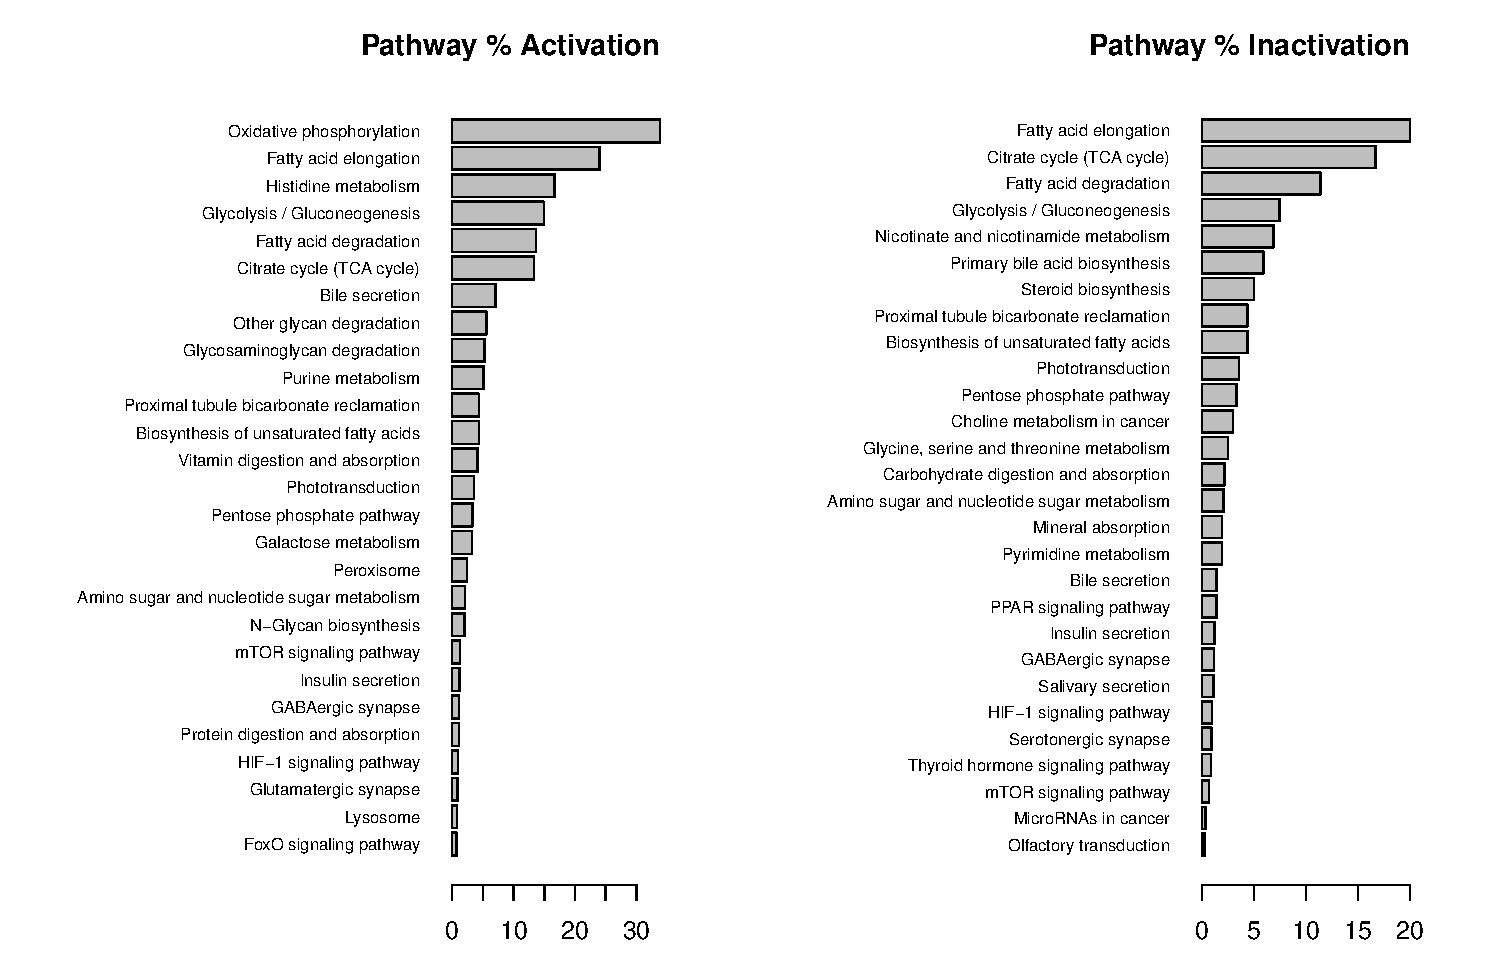
\includegraphics[width=\textwidth]{neuroprotective/Healthy2Inflammated}
\end{center}
\caption{Metabolic pathways affected by metabolic inflammation. Percentage of activation and inactivation was calculated in comparison with genes associated with each pathway in the KEGG database}
\label{h2i}
\end{figure}

L-serine and L-asparagine uptake increase may be related to the cell survival process that switches cellular metabolism to be highly dependent of nonessential amino acids available in extracellular space such as glutamine, serine, glycine, arginine, and asparagine \cite{Green2014}. Moreover, under the inflamed scenario, our astrocyte model release a very small amount of prostaglandin D2. The release of this prostaglandin was previously associated to induce the depolarization and potentiate the actions of simultaneously applied transmitters such as GABA, taurine, glutamate, and aspartate in astrocytes \cite{Murphy1988}.\\

In our inflamed scenario, astrocytes activate the 46.6\% of model reactions (5.6\% less than healthy scenario) and affect the biomass flux rate of 586 reactions in comparison with the healthy scenario. Main metabolic changes occur in the activation of oxidative phosphorylation, histidine metabolism, and fatty acid degradation pathways; as well as an inactivation of TCA and glycolysis pathways (Fig. \ref{h2i}). Inflammation affects in a negative way all metabolic objective functions evaluated except the release of D-serine. In comparison to the healthy scenario, growth rate over DMEM medium decrease in a 15.6\%, the catch of cysteine to produce reduced glutathione in a 59.3\%, conversion of glucose to ATP in a 72\%, and to lactate in a 74.4\%; finally, conversion of extracellular glutamate in glutamine reduces in a 67.7\% (Fig. \ref{Effects}). \\

\begin{table}[h]
\caption{Set of reactions with pro-inflammatory potential identified through a sensibility analysis over inflamed scenario.}
\label{Proinflammatory}
\begin{tabular}{>{\centering\arraybackslash}m{2.5cm}  m{8cm}  >{\centering\arraybackslash}m{1cm} >{\centering\arraybackslash}m{1cm} >{\centering\arraybackslash}m{2cm}}
\hline
ID & REACTION DESCRIPTION & H. FLUX & I. FLUX & FOLD CHANGE \\
\hline
\hline
FTCD & Formimidoyltransferase cyclodeaminase & 0.39 & 1.28 & 2.28 \\
H2Otm & H2O transport mitochondrial & -0.26 & 2.44 & 10.44 \\
\hline
\end{tabular}
\end{table}

Based on performed sensibility analysis, we identify two pro-inflammatory reactions candidate to be knocked out (Table \ref{Proinflammatory}), that when being blocked increases the value of the objective function above the maximum value set (in an 11.45\% and 5.14\% respectively) for the inflammated scenario. Reactions are associated to the formimidoyl-transferase cyclodeaminase (FTCD) enzyme and the Aquaporin-8, a water transport protein.\\

\begin{table}[h]
\caption{Set of reactions with anti-inflammatory potential identified through a sensibility analysis over inflamed scenario.}
\label{Antiinflammatory}
\begin{center}
\begin{tabular}{>{\centering\arraybackslash}m{2.5cm}  >{\arraybackslash}m{8cm}  >{\centering\arraybackslash}m{1cm}  >{\centering\arraybackslash}m{1cm}  >{\centering\arraybackslash}m{2cm}}
\hline
ID & REACTION DESCRIPTION & H. FLUX & I. FLUX & FOLD CHANGE \\
\hline
\hline
AKGMALtm& $\alpha$-ketoglutarate/malate transporter&-0.17&-1.3&-6.85\\ 
%\hline
NADH2\_u10m&NADH dehydrogenase mitochondrial &0.12&0.37&2.17\\ 
%\hline
r0639&Lauroyl-CoA:\newline acetyl-CoA C-acyltransferase.&0.02&0.09&4.04\\ 
%\hline
r0653&cMyristoyl-CoA:\newline acetyl-CoA C-myristoyl transferase&0.02&0.09&4.04\\ 
%\hline
r0714&(S)-3-Hydroxyhexadecanoyl-CoA:\newline NAD$^+$ oxidoreductase&0.02&0.09&4.04\\ 
%\hline
r0716&(S)-3-Hydroxyhexadecanoyl-CoA hydrolyase &0.02&0.09&4.04\\ 
%\hline
r0718&(S)-3-Hydroxytetradecanoyl-CoA:\newline NAD+ oxidoreductase&0.02&0.09&4.04\\ 
%\hline
r0720&(S)-3-Hydroxytetradecanoyl-CoA hydrolyase&0.02&0.09&4.04\\ 
\hline
\end{tabular}
\end{center}
\end{table}

FTCD enzyme, previously reported as over-expressed in high-fat diets \cite{Fernando2013}, contribute with one-carbon units from histidine degradation to the folate pool \cite{Varemo2015}. In turn, the Aquaporin 8, generally  associated to ammonia and water transport \cite{Saparov2007}, has been proposed as a biomarker for inflammation processes where was in contrary way to our observations, highly correlated to cellular defence against severe oxidative stress \cite{TeVelde2008}.\\

As well as pro-inflammatory reactions, eight anti-inflammatory reactions were identified. Identified reactions (Table \ref{Antiinflammatory}) have a change between scenarios greatest equal to 2-fold and when being blocked decreased, even more, the value of the objective function in comparison with the healthy scenario. The majority of identified reactions (r0639, r0653, r0714, r0716, r0718 and r0720) are involved in the fatty acid elongation in mitochondria through acyl-COA association \cite{Landriscina1972}. The elongation system, is responsible for the addition of two carbon units to the carboxyl end of a fatty acid chain, and play an important role in the maintenance of membrane lipid composition as well as in the generation of precursors for cell signaling molecules (such as eicosanoids and sphingosine-1 phosphate), energy production, and other unknown pathways involving with cancer growth. \cite{Tamura2009}.

\subsection*{Medicated Scenario}
The inflamed scenario with the 279 reactions associated with tibolone and estradiol-derivated compounds metabolism, defined as our medicated scenario displays several neuroprotective effects. Medicated scenario increase the demand of L-aspartate and in turn decreases the demand for L-asparagine, L-glutamate and the release of L-glutamine in comparison to the inflamed scenario (Fig. \ref{Exchanges}).\\

\begin{figure}[h]
\begin{center}
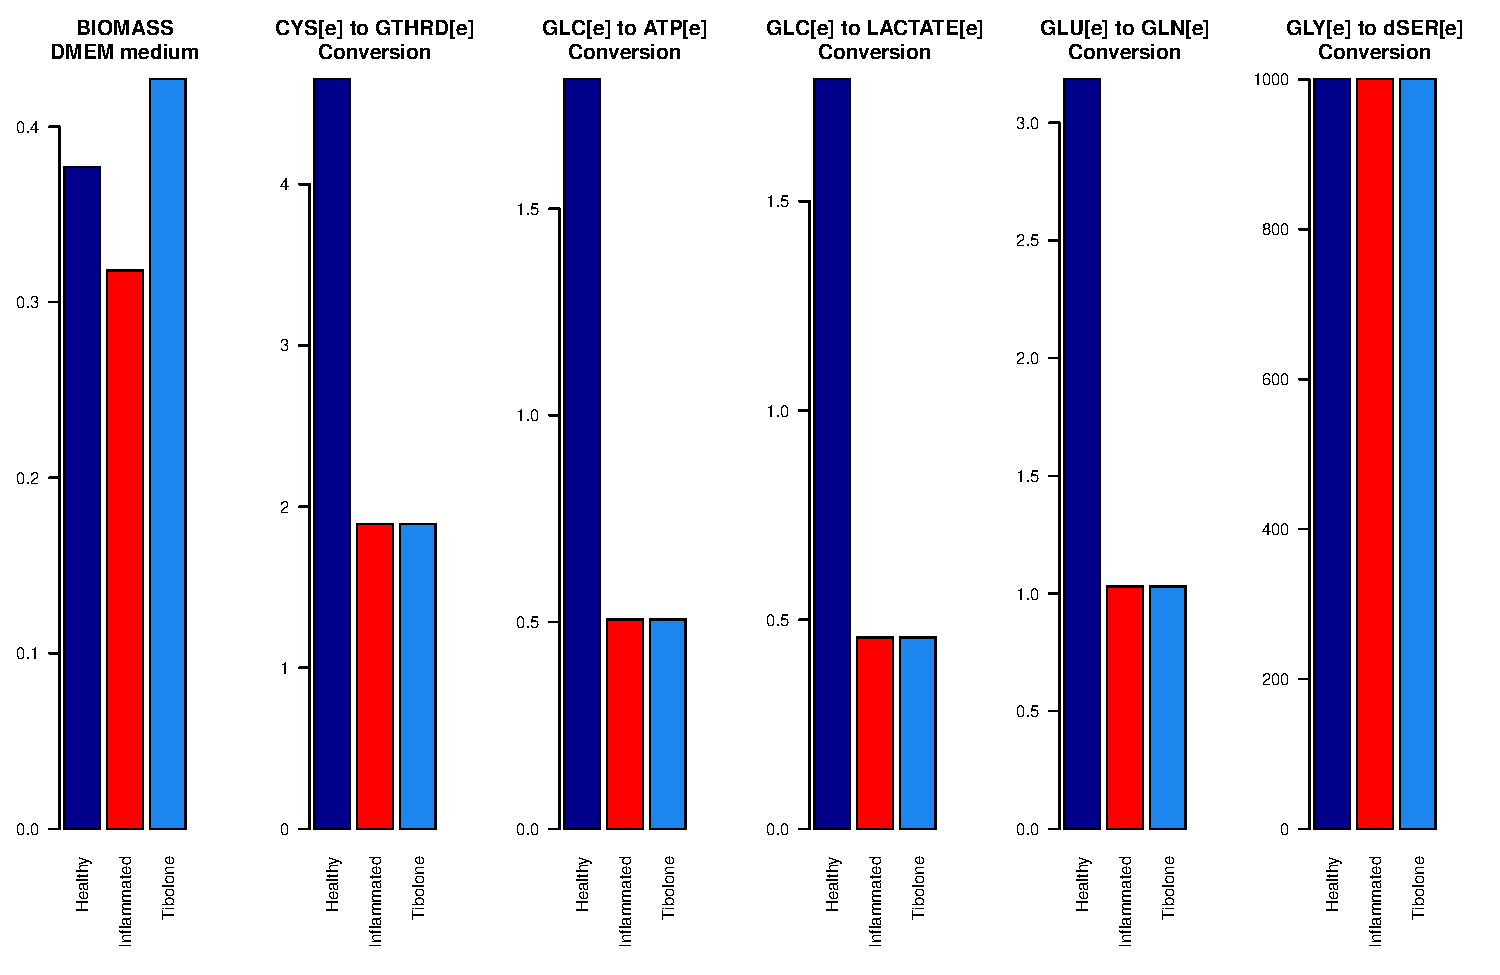
\includegraphics[width=\textwidth]{neuroprotective/Effects}
\end{center}
\caption{The response of the main astrocytes metabolic capabilities to different modeled scenarios.}
\label{Effects}
\end{figure}

The reduction of L-glutamate and L-glutamine uptake/release rate mediated by Tibolone effects could be associated with a neuroprotective effect through a reduction of neurotoxicity mediated by L-glutamate in astrocytes \cite{Petrelli2016}. L-glutamate is a contributing factor in neuronal damage induced by inflammation, traumatic brain injury, stroke, and in most of the chronic neurodegenerative diseases, such as PD and AD \cite{Ahlemeyer2002}.\\

In our medicated scenario, astrocytes activate 46.6\% of model reactions, equal than in inflamed scenario. Nevertheless, tibolone effects affect the biomass flux rate of 948 reactions in comparison with the inflamed scenario; main metabolic changes occurs through the activation of several metabolic pathways with neuroprotective actions associated such as taurine metabolism, which has been shown to be tissue-protective in many models of oxidant-induced injury \cite{Schuller-Levis2003}, gluconeogenesis which is accelerated and facilitate the conversion of fatty acids into ketone bodies under steroid-mediated effects \cite{Amen-Ra2006}, calcium and PPAR signaling pathways (Fig. \ref{I2T}).\\

\begin{figure}[h]
\begin{center}
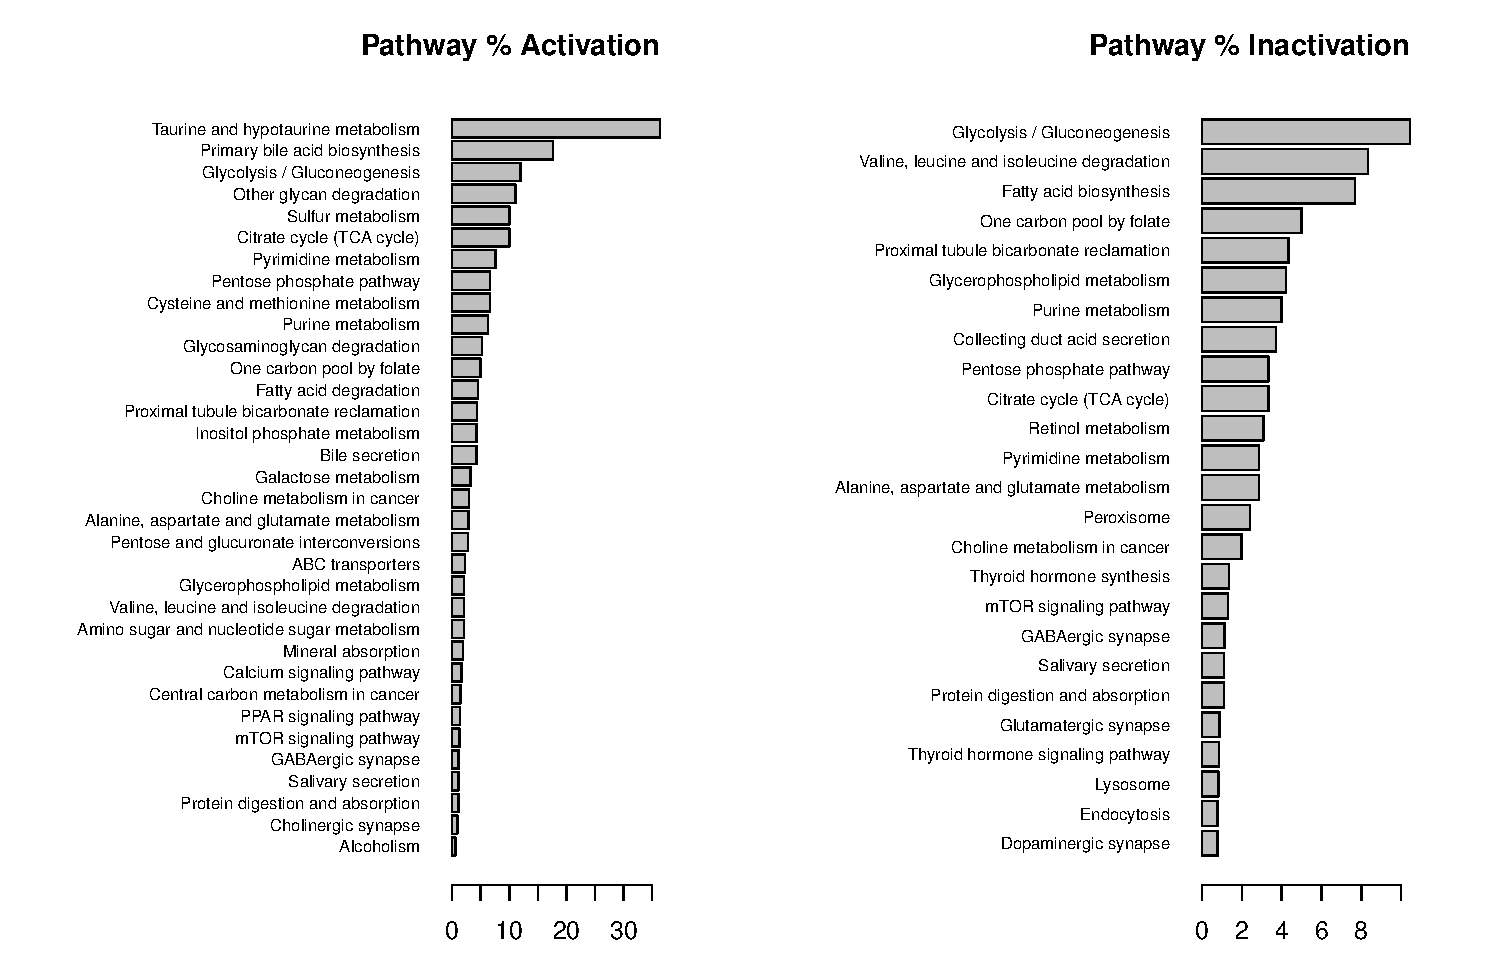
\includegraphics[width=\textwidth]{neuroprotective/Inflammated2Tibolone}
\end{center}
\caption{Metabolic pathways affected by tibolone effects over inflamed scenario. Activation and inactivation percentage was measured in comparison with genes associated to each pathway in the KEGG database
}
\label{I2T}
\end{figure}

Tibolone does not show directly effect over the main associated neuron-supportive capabilities (Table \ref{Reactions}) by affected by inflammation, however, it shows a high related activity as a potentiator of growth rate (Fig. \ref{Effects}). An increase of growth rate (13.26\% higher than in healthy scenario) could be associated with an increase in cell viability or as an increase in the proliferative potential in cells \cite{Feist2010}. Due that proliferative potential was not evidenced in the inflamed scenario, this proliferative potential must not be associated with astrogliosis mediated proliferation in astrocytes \cite{Takuma2004}. However, it could be associated with the proliferative side effect of steroid compounds as was previously reported in other cell types where tibolone was tested in wet lab \cite{Colditz1993,Colditz1995}. \\

\begin{table}[h]
\caption{Set of reactions associated with tibolone required to execute its neuroprotective effects. Reactions were identified through a sensibility analysis over the medicated scenario.}	
\label{tibolone}
\begin{center}
\begin{tabular}{rll}
\hline
ID & REACTION DESCRIPTION & GENES IN ASTROCYTE DATA\\
\hline
\hline
r0739 & Alcohol Dehydrogenase & ADH4, ADH5, ADH7\\
r2518 & ATP-binding Cassette (ABC) & ABCD3\\
RE1804M &	Cholestanetriol 26-monooxygenase& CYP27A1 \\
RE1807M & Cholestanetriol 26-monooxygenase& CYP27A1 \\
\hline
\end{tabular}
\end{center}
\end{table}

Based on performed sensibility analysis over the 289 reactions associated with tibolone and estradiol-derivated compounds metabolism, we identify a set of four reactions that when being individually knocked out, block entirely the tibolone effects (Table \ref{Tibolone}). Identified reactions are catalyzed by an alcohol dehydrogenase (E.C. 1.1.1.1) and a Cytochrome P450 associated with the PPAR signaling pathway. Both enzymes were previously reported with ROS reduction through redox reactions mediated by alcohol dehydrogenase (ADH) and posterior release associated to a cytochrome P450 \cite{Pessayre2001, Sun2009}. 

\section{Conclusion}
In this work, a tissue-specific metabolic network for mature astrocyte has been developed, and three different scenarios were modeled. Modeled scenarios allowed identify the metabolic changes between a healthy and an inflamed scenario as well as from an inflamed to a tibolone medicated scenario. The model was capable of yielding results which were in correspondence to the experimentally proved metabolic processes \cite{Das2010,Liu2013}. From our study, adverse effects associated with the increase of palmitate uptake were described based on exchange, metabolite production, and metabolic pathways perturbed under inflammatory response. Sensibility analysis performed through constrained-based modeling approach and FBA methods permitted recognize two possible reactions and their associated enzymes susceptible to be knocked out to reduce inflammatory processes.\\

Based on literature reports we modeled a tibolone medicated scenario used to identify and describe the neuroprotective effects of this synthetic neurosteroid under an inflamed scenario in astrocytes; our main results suggest that tibolone execute their neuroprotective effects through a reduction of neurotoxicity mediated by L-glutamate in astrocytes. L-glutamate \cite{Petrelli2016}. We also found a tibolone associated increase in growth rate probably in concordance to previously reported side effects of steroids in other human cell types \cite{Colditz1993,Colditz1995}. Identified enzyme associated reactions with tibolone effects and their action mechanisms are highly consistent with reported previously by our associated wet lab \cite{Avila-Rodriguez2014, Avila-Rodriguez2016}. 